\section[Appendix]{Appendix}
\label{sec:app_a}

\subsection{Project Repository}
\href{https://github.com/bhavik-knight/5580-a6-anomaly-detection-nsp}{GitHub repository}

\subsection{Supplementary Tables}
\begin{table}[H]
\centering
\caption{Forecasting metrics by region and model (latest notebook run)}
\label{tab:app_forecast_metrics}
\begin{tabular}{lccc|ccc}
\toprule
\multirow{2}{*}{Region} & \multicolumn{3}{c|}{Prophet} & \multicolumn{3}{c}{Advanced-LSTM-Optuna} \\
\cmidrule(lr){2-4} \cmidrule(lr){5-7}
& MAE & RMSE & MAPE (\%) & MAE & RMSE & MAPE (\%) \\
\midrule
Annapolis Valley & 20.16 & 48.99 & 22.00 & 25.43 & 52.22 & 26.00 \\
Cape Breton      & 36.36 & 85.21 & 20.00 & 45.70 & 91.09 & 21.00 \\
Halifax          & 93.99 & 213.15 & 23.00 & 131.58 & 238.77 & 25.00 \\
Pictou County    & 12.56 & 28.13 & 28.00 & 18.69 & 32.20 & 37.00 \\
South Shore      & 17.07 & 39.34 & 27.00 & 20.83 & 41.97 & 33.00 \\
\bottomrule
\end{tabular}
\end{table}
\begin{table}[H]
\centering
\caption{Global anomaly detection summary by method}
\label{tab:app_global_method_summary}
\begin{tabular}{lccc}
\toprule
Method & Total Anomaly & \% of Total Rows & \% within Method Flags \\
\midrule
IQR & 6596 & 1.51 & 19.60 \\
Isolation Forest & 8765 & 2.00 & 26.05 \\
LSTM Autoencoder & 14912 & 3.40 & 44.32 \\
Z-Score & 3373 & 0.77 & 10.02 \\
\bottomrule
\end{tabular}
\end{table}
\begin{table}[H]
\centering
\caption{Region-wise anomaly summary (total anomalies by method)}
\label{tab:app_region_method_summary}
\begin{tabular}{lcccc}
\toprule
Region & Z-Score & IQR & Isolation Forest & LSTM Autoencoder \\
\midrule
Annapolis Valley & 720 & 1093 & 1753 & 3151 \\
Cape Breton      & 692 & 1644 & 1753 & 2698 \\
Halifax          & 687 & 1304 & 1753 & 2981 \\
Pictou County    & 601 & 1378 & 1753 & 2934 \\
South Shore      & 673 & 1177 & 1753 & 3148 \\
\bottomrule
\end{tabular}
\end{table}

\subsection{Supplementary Figures from Modeling Outputs}

\begin{figure}[H]
\centering
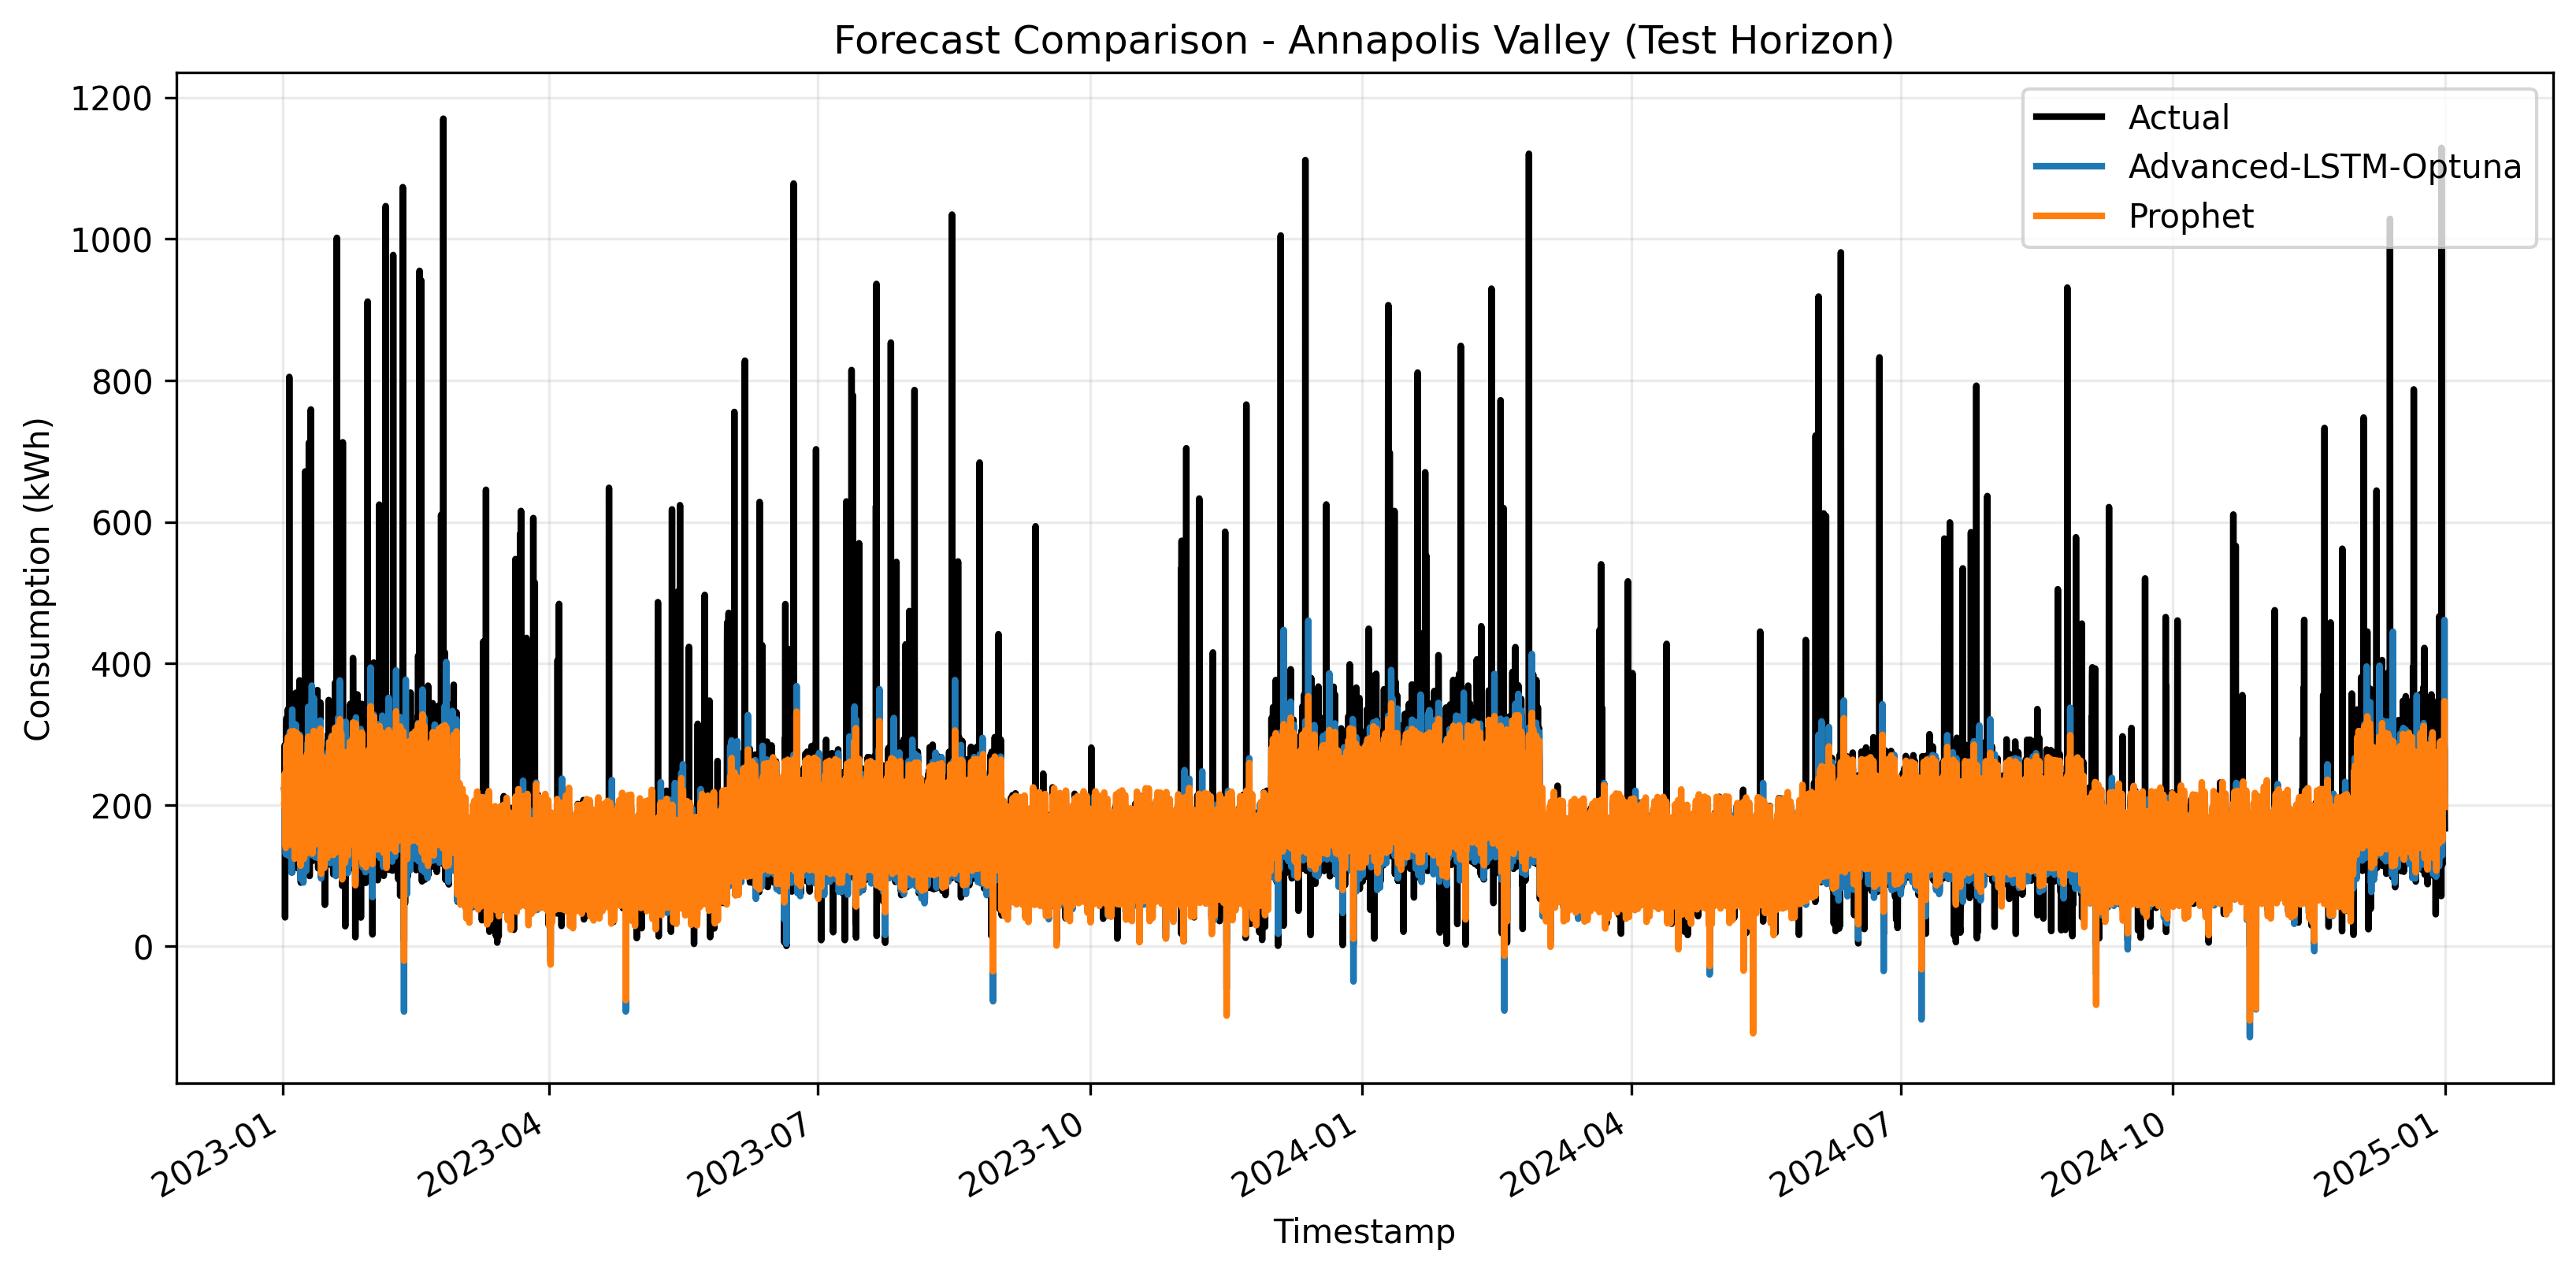
\includegraphics[width=0.95\textwidth]{figures/forecast_plot.png}
\caption{Forecast comparison of actual consumption vs Prophet and Advanced-LSTM-Optuna (test horizon).}
\label{fig:app_forecast_plot}
\end{figure}

\begin{figure}[H]
\centering
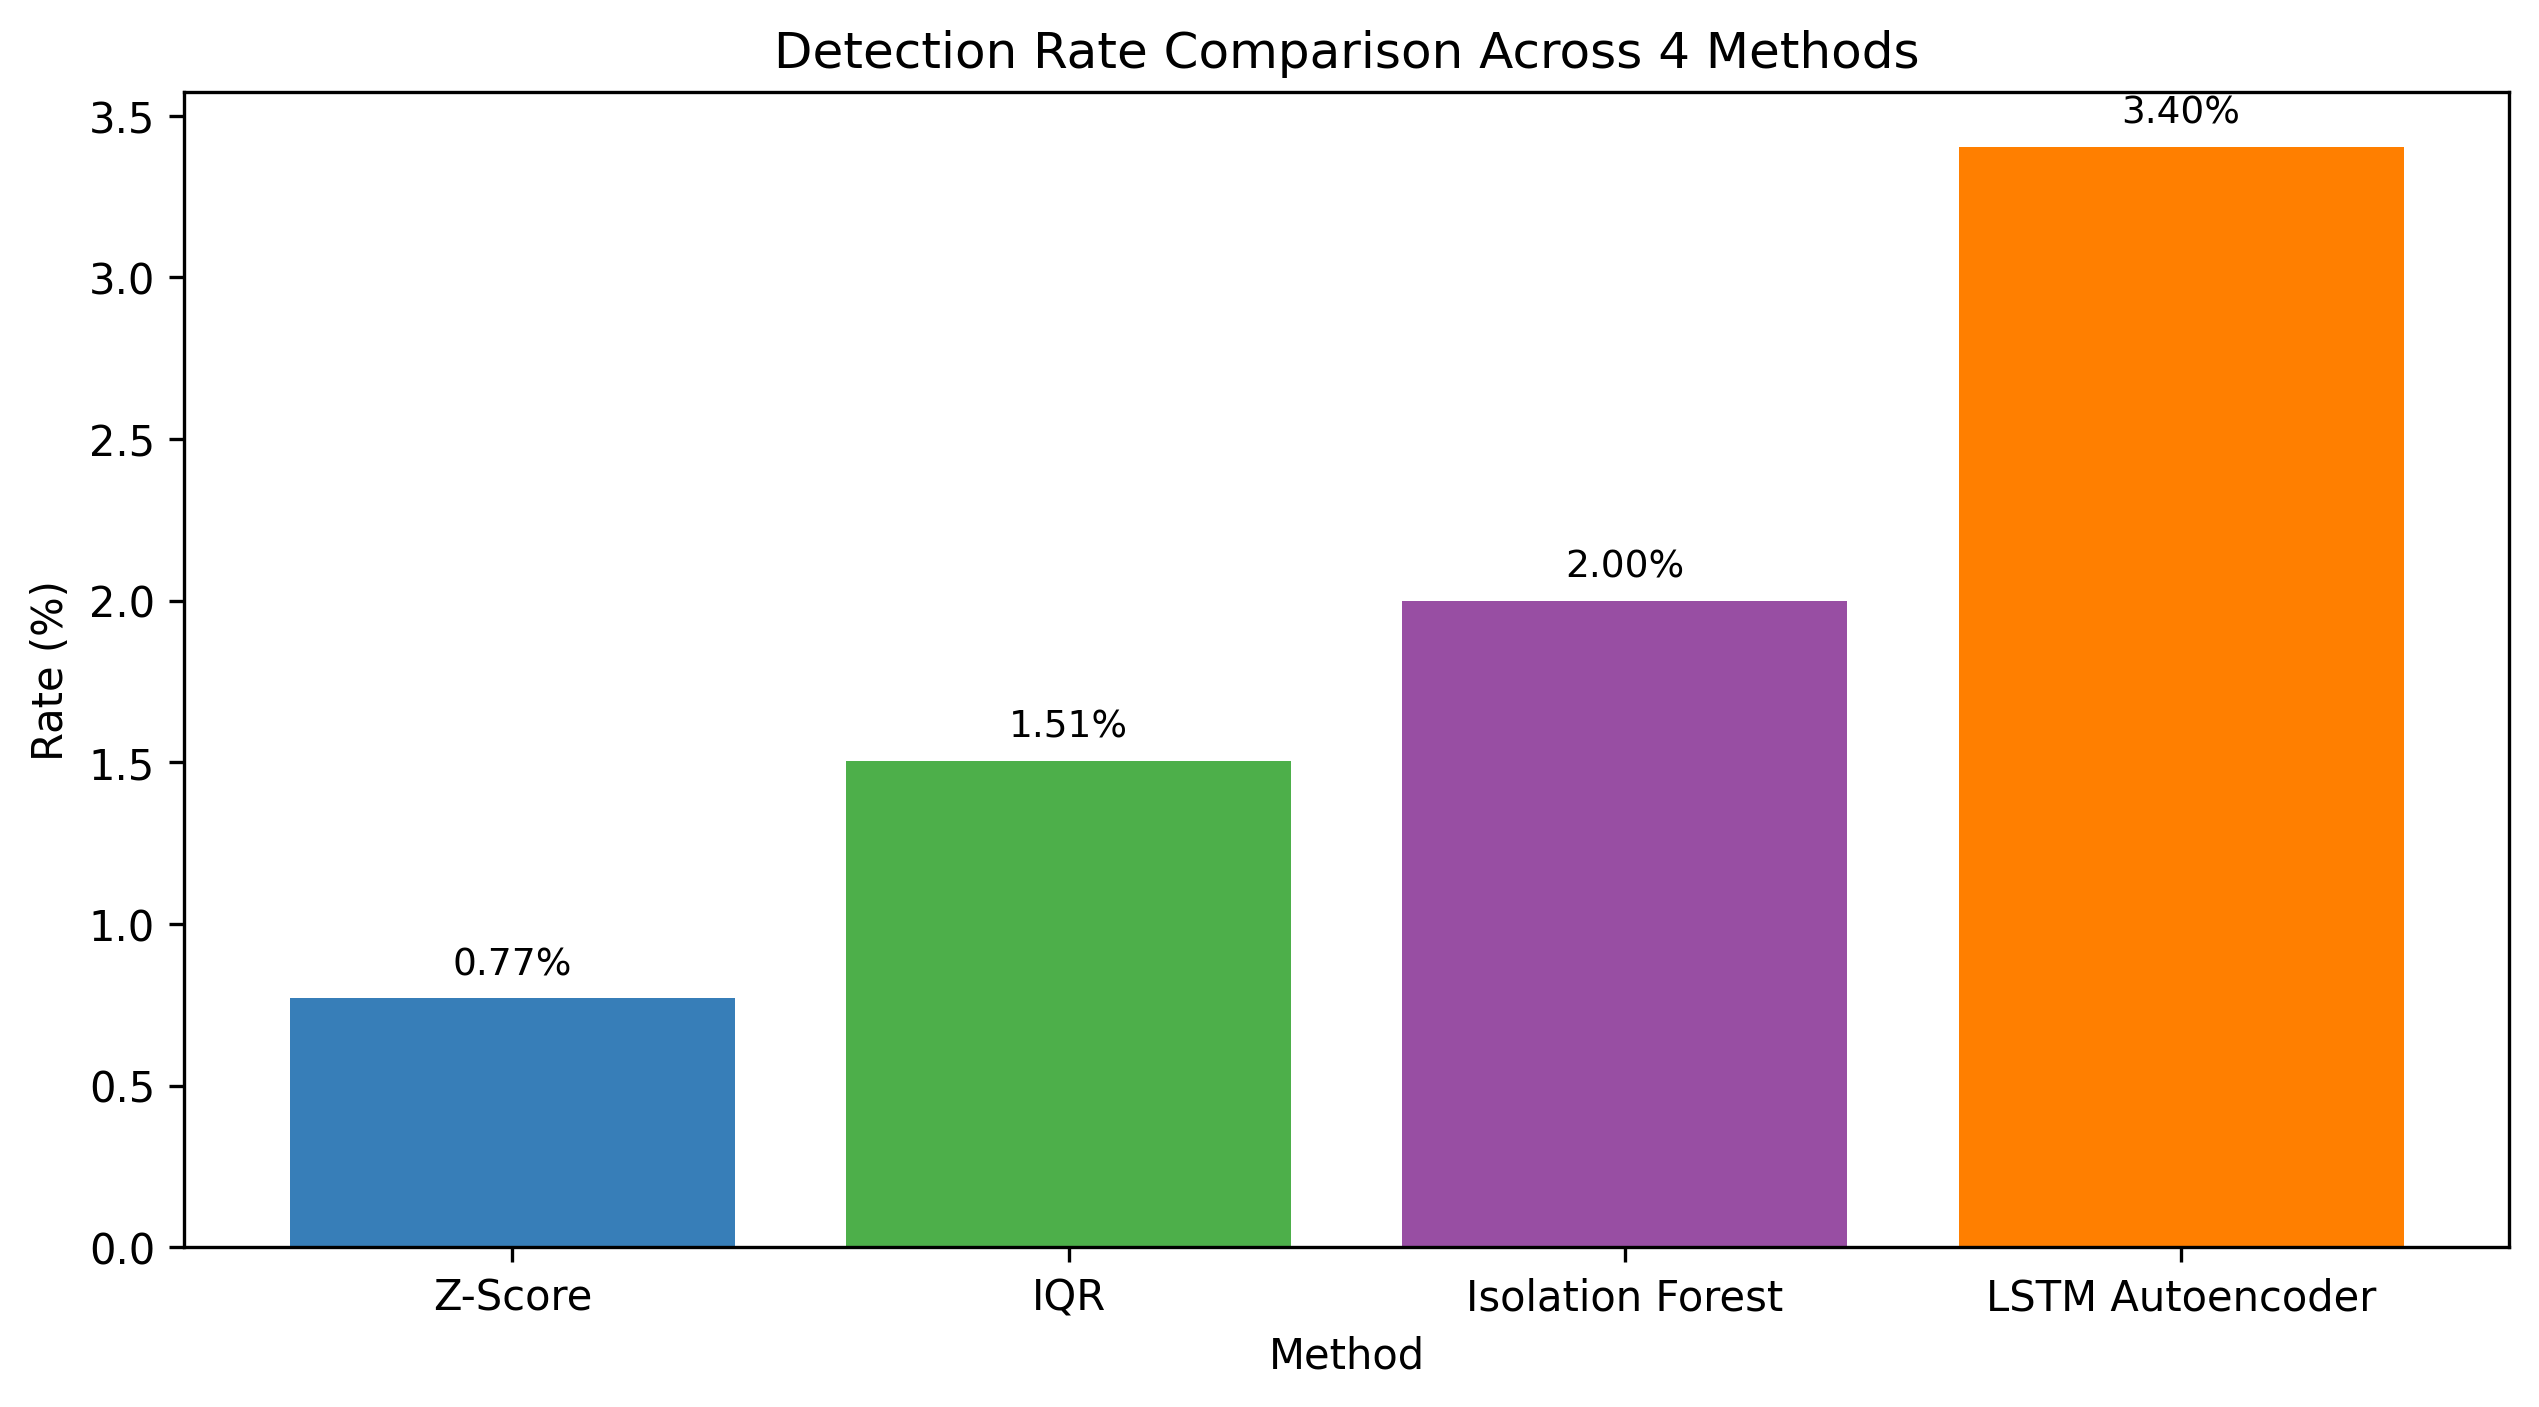
\includegraphics[width=0.95\textwidth]{figures/anomaly_detection_rate_4method_comparison.png}
\caption{Final 4-method anomaly detection rate comparison.}
\label{fig:app_anomaly_4method}
\end{figure}

\begin{figure}[H]
\centering
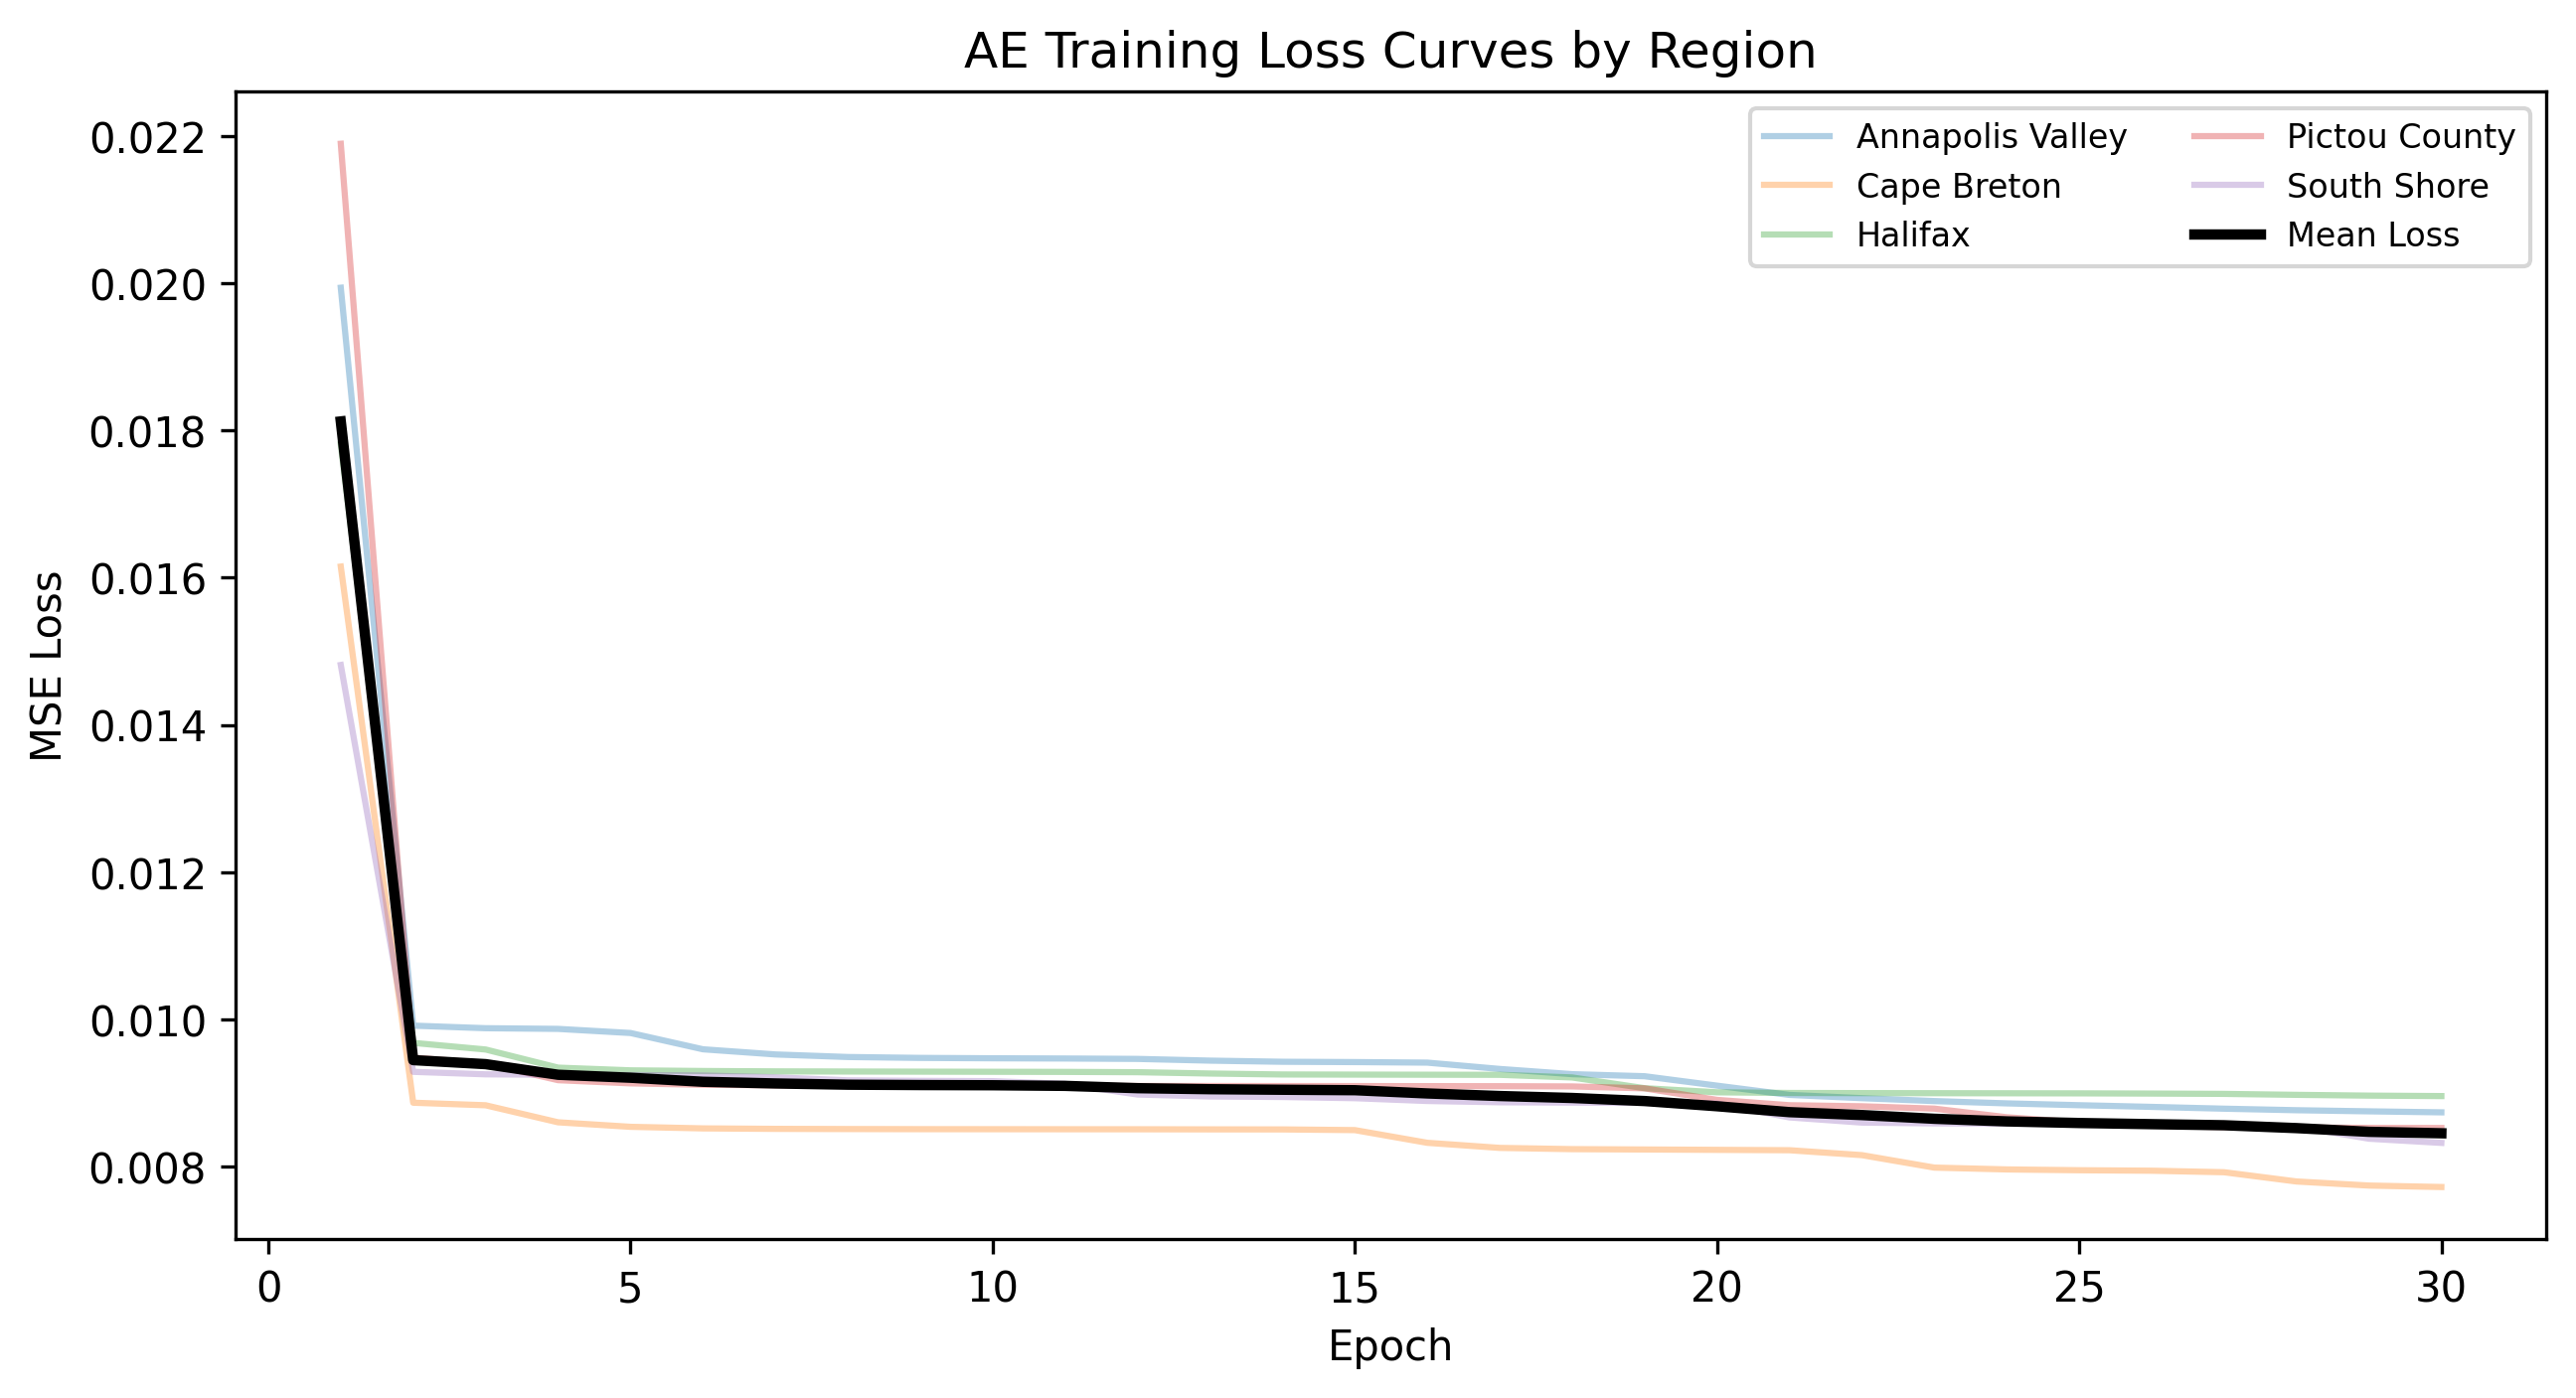
\includegraphics[width=0.9\textwidth]{figures/ae_training_loss_curve.png}
\caption{Autoencoder training loss curves across regions.}
\label{fig:app_ae_loss}
\end{figure}

\begin{figure}[H]
\centering
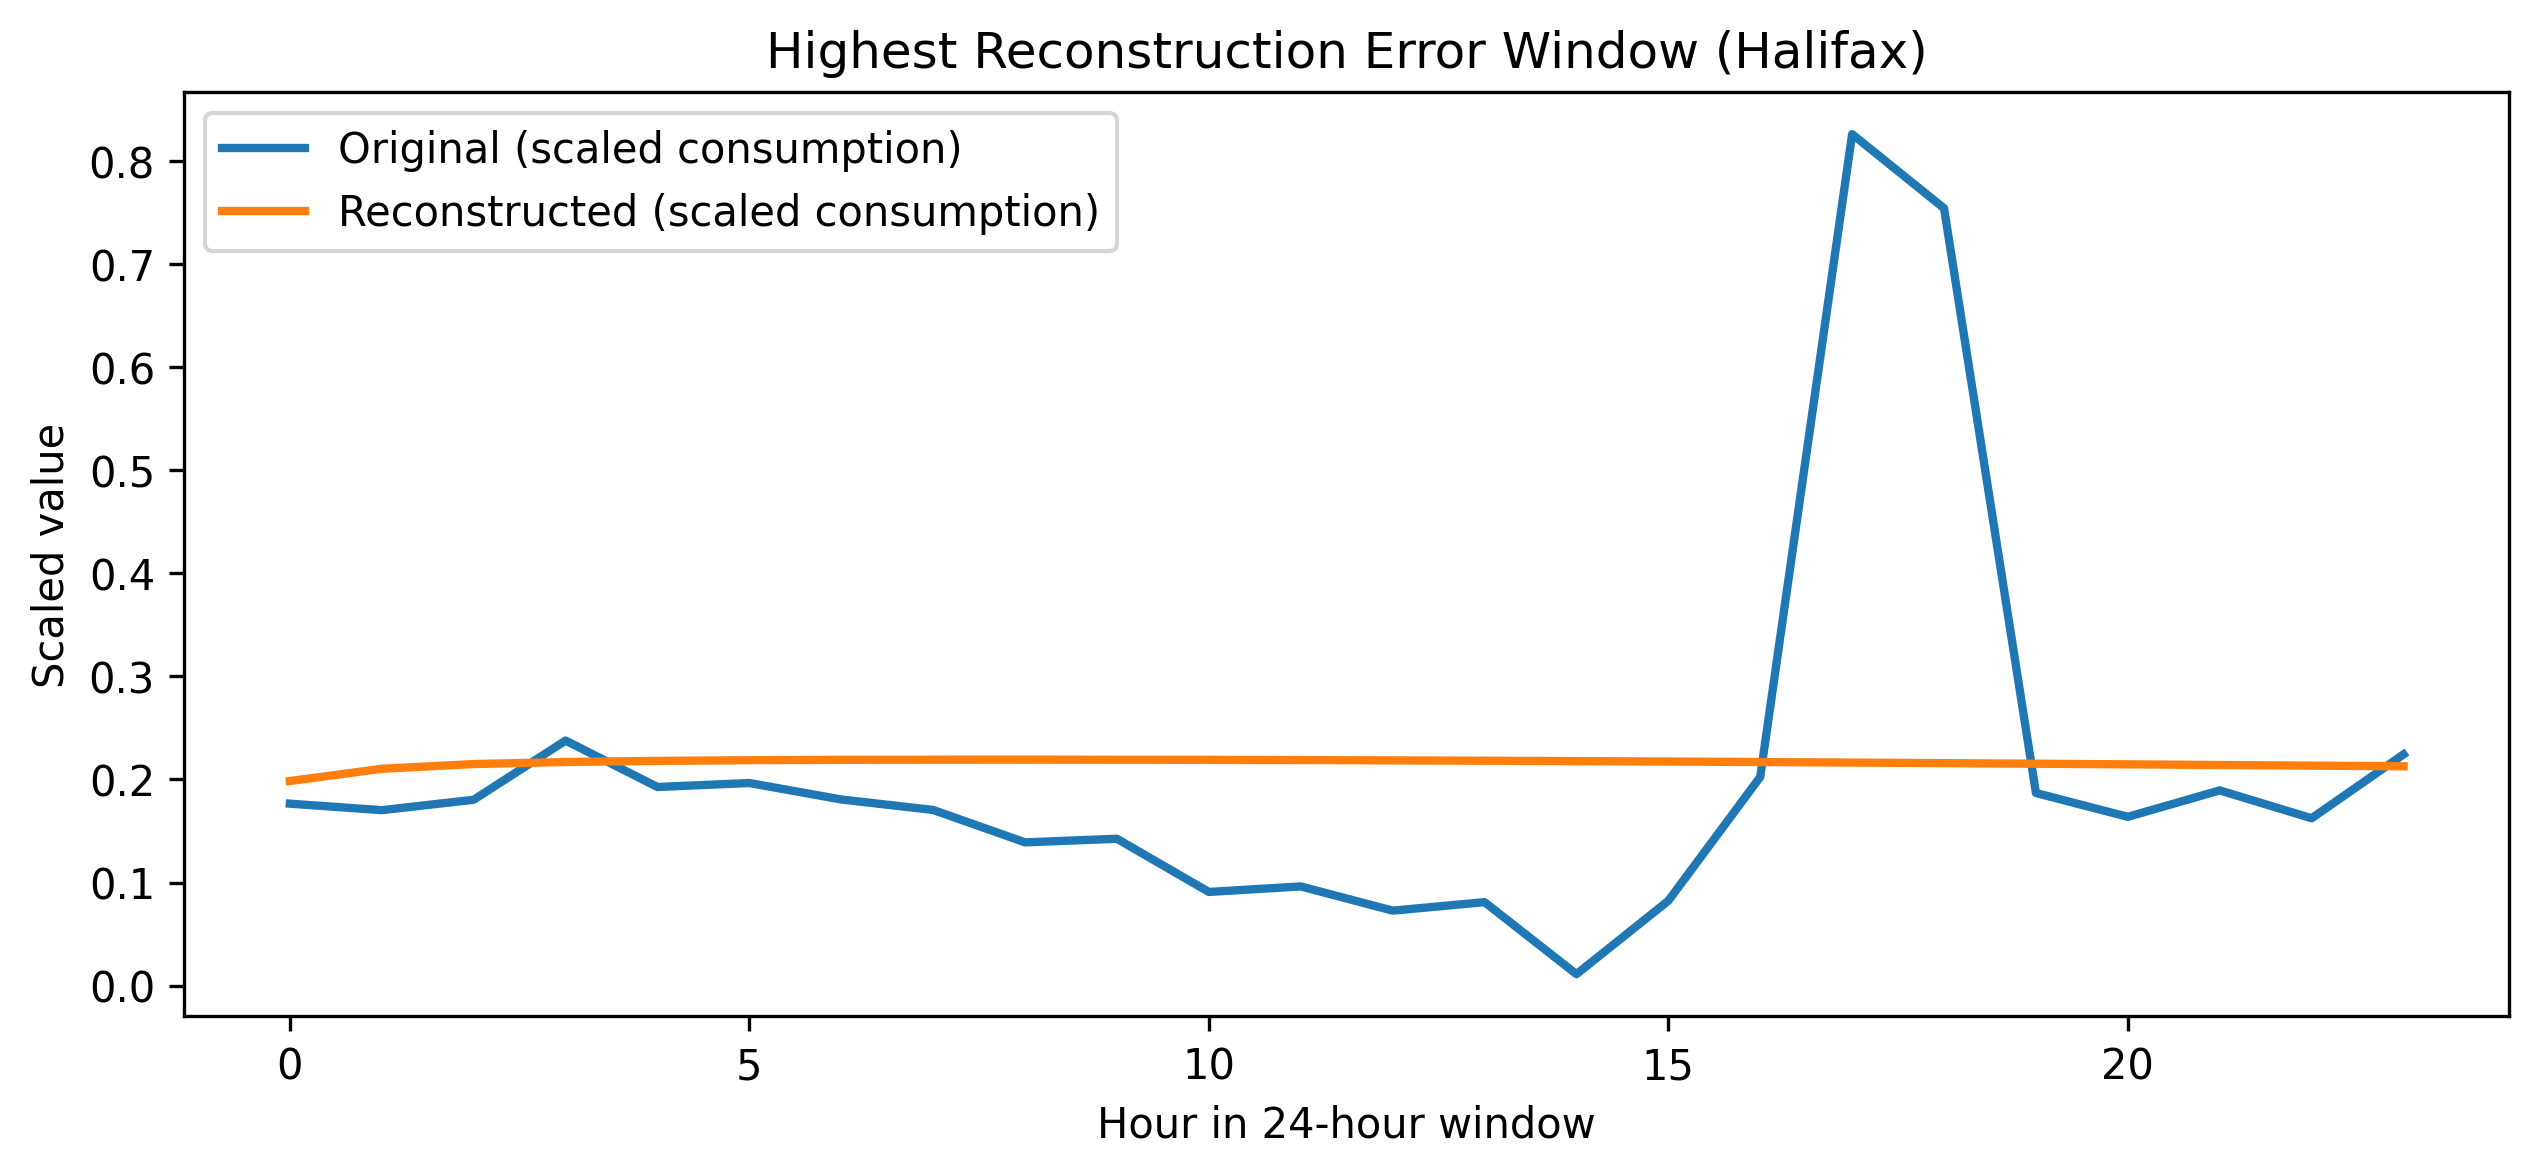
\includegraphics[width=0.9\textwidth]{figures/ae_original_vs_reconstructed.png}
\caption{Autoencoder reconstruction example for highest-error sequence window.}
\label{fig:app_ae_reconstruction}
\end{figure}

\begin{figure}[H]
\centering
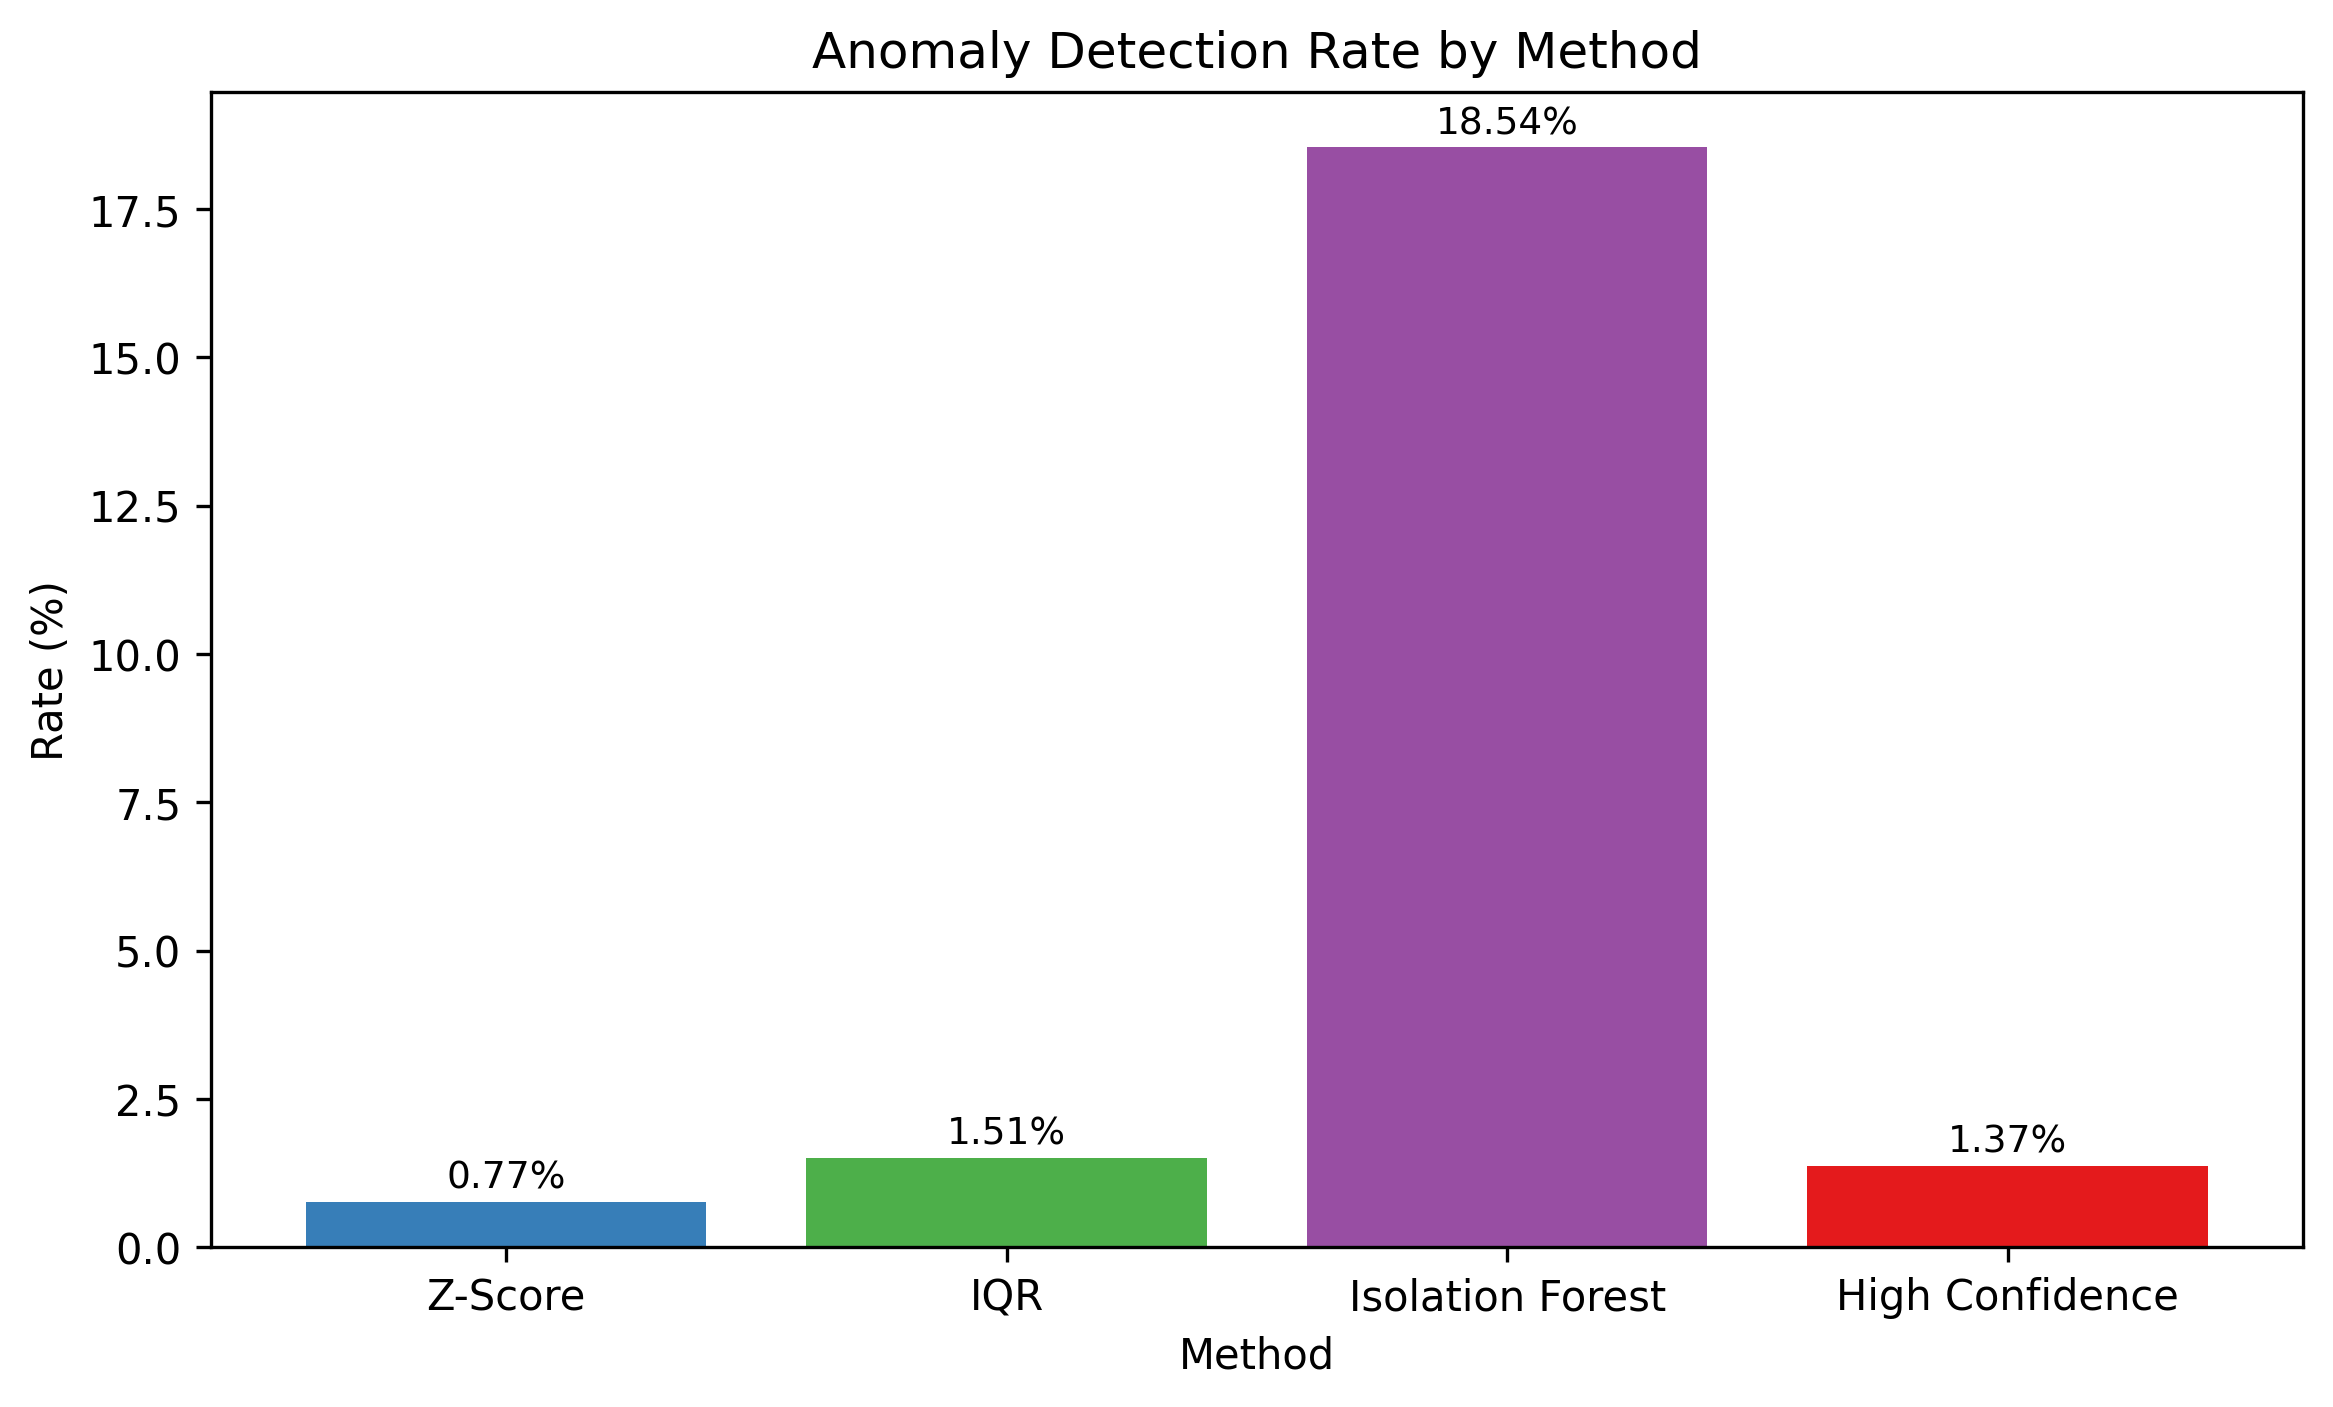
\includegraphics[width=0.85\textwidth]{figures/anomaly_detection_rate_comparison.png}
\caption{Intermediate anomaly detection rate comparison.}
\label{fig:app_anomaly_intermediate}
\end{figure}

\begin{figure}[H]
\centering
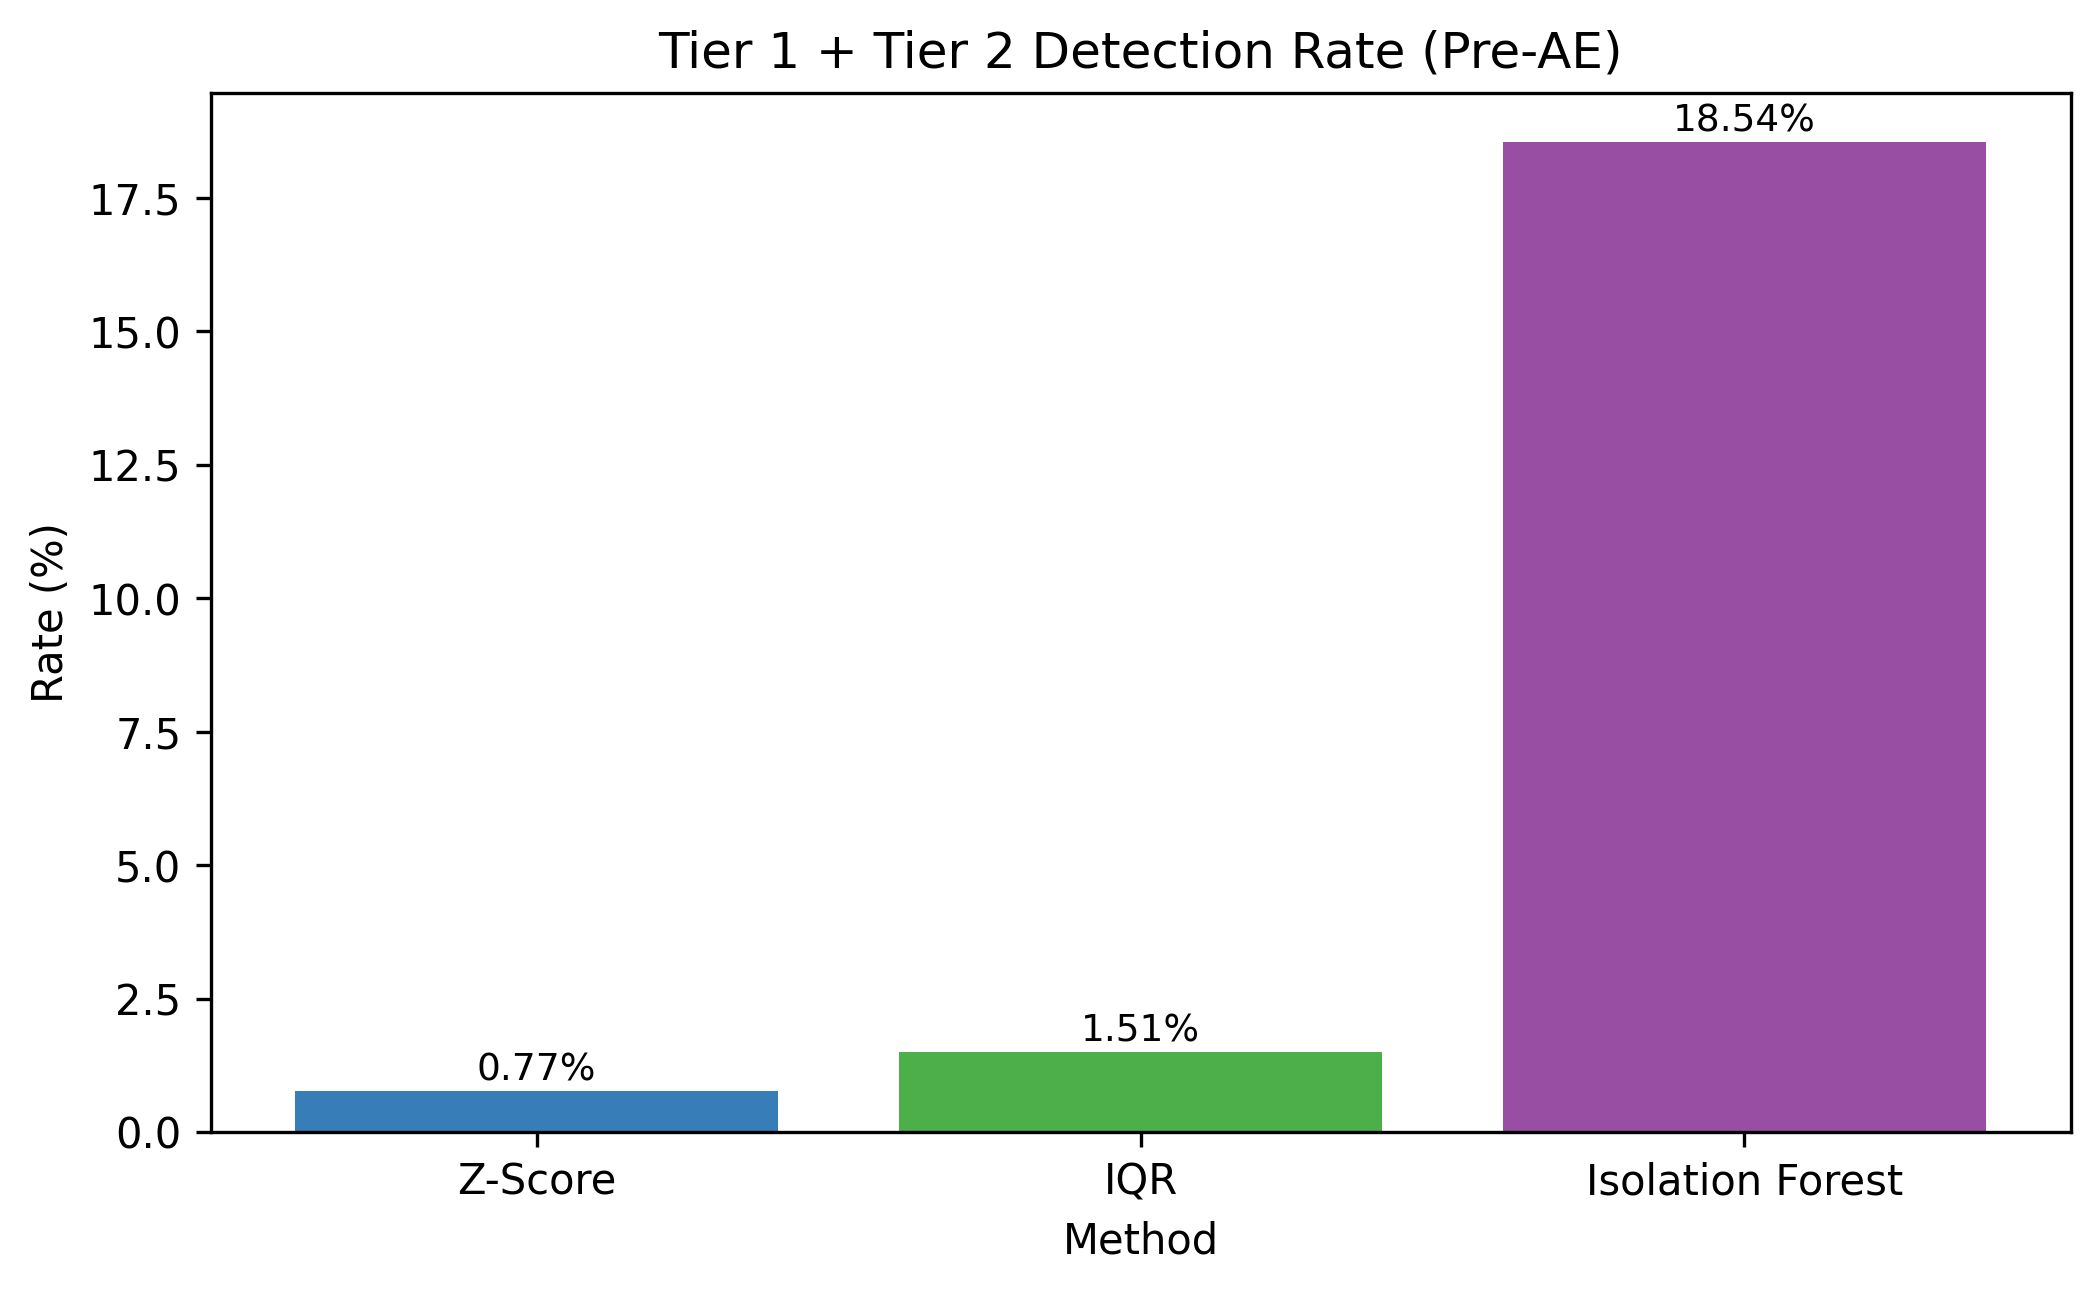
\includegraphics[width=0.85\textwidth]{figures/tier12_detection_rate_comparison.png}
\caption{Tier 1 and Tier 2 detector comparison (pre-autoencoder).}
\label{fig:app_tier12_compare}
\end{figure}

\begin{figure}[H]
\centering

\includegraphics[width=0.9\textwidth]{figures/Feature_Correlation_Heatmap.png}
\caption{Feature correlation heatmap from engineered feature space.}
\label{fig:app_feature_corr}
\end{figure}

\begin{figure}[H]
\centering
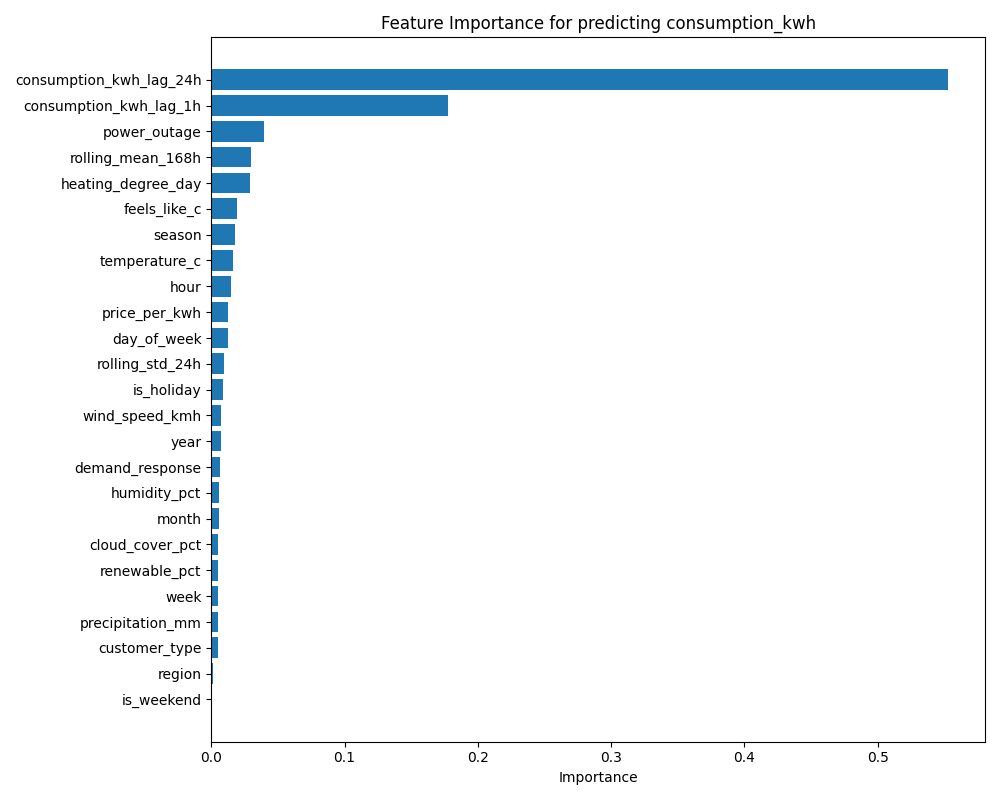
\includegraphics[width=0.85\textwidth]{figures/feature_importance_plot_25.png}
\caption{Feature importance output (configuration 25).}
\label{fig:app_feat_imp_25}
\end{figure}

\begin{figure}[H]
\centering
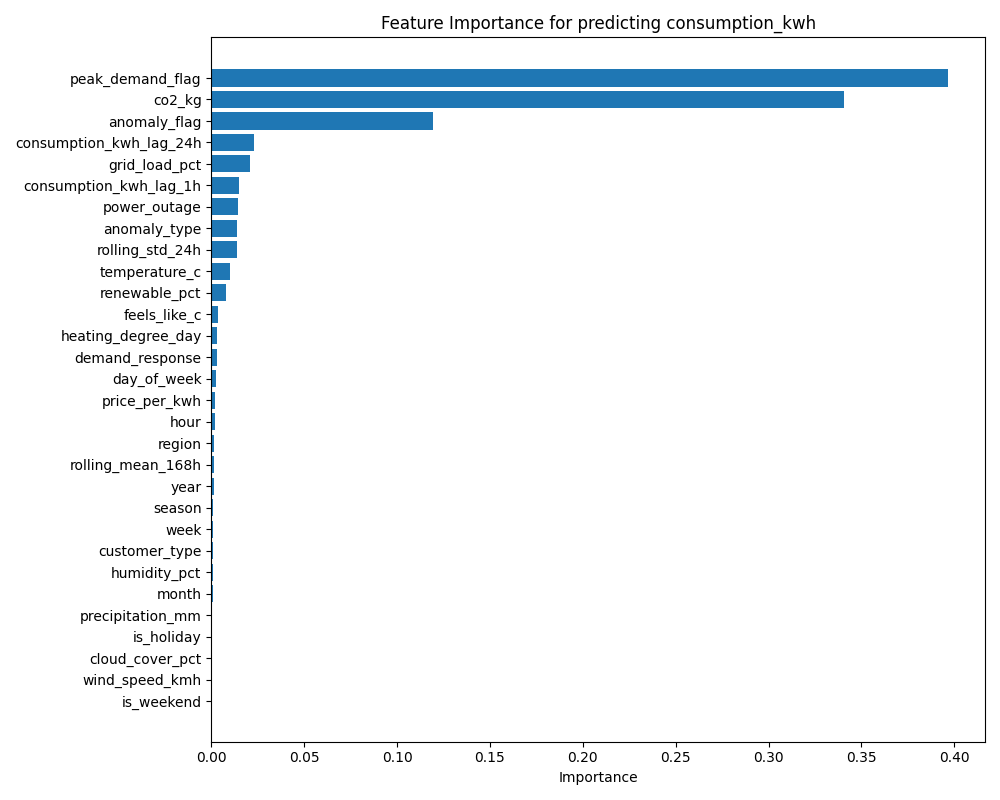
\includegraphics[width=0.85\textwidth]{figures/feature_importance_plot_30.png}
\caption{Feature importance output (configuration 30).}
\label{fig:app_feat_imp_30}
\end{figure}

\begin{figure}[H]
\centering

\includegraphics[width=0.85\textwidth]{figures/customer_vs_consumption.png}
\caption{Customer-type versus consumption relationship.}
\label{fig:app_customer_vs_consumption}
\end{figure}

\begin{figure}[H]
\centering

\includegraphics[width=0.85\textwidth]{figures/hour_vs_consumption.png}
\caption{Hourly consumption pattern visualization.}
\label{fig:app_hour_vs_consumption}
\end{figure}

\begin{figure}[H]
\centering

\includegraphics[width=0.85\textwidth]{figures/temp_vs_consumption.png}
\caption{Temperature versus consumption relationship.}
\label{fig:app_temp_vs_consumption}
\end{figure}

\begin{figure}[H]
\centering

\includegraphics[width=0.95\textwidth]{figures/pair_plot.png}
\caption{Multivariate pair plot used for exploratory assessment.}
\label{fig:app_pair_plot}
\end{figure}
